%\documentclass[russian,english,10pt,a5paper,reqno]{amsart}
%\documentclass[russian,english,10pt,a4paper,reqno]{article}
%\documentclass[russian,english,11pt,b5paper,reqno,dviphfm]{amsbook}
%\documentclass[russian,english,10pt,a5paper,reqno,dviphfm]{amsbook}
%\documentclass[russian,english,10pt,a5paper,reqno,dviphfm]{amsbook}
\documentclass[russian,english,18pt,a4paper,reqno,dviphfm]{article}


%%\usepackage[pdftex,a5paper]{hyperref}
\usepackage[headings]{fullpage}
%\usepackage{fancyhdr}
%%\setlength{\textwidth}{114mm}
%%\setlength{\linewidth}{114mm}
%%\setlength{\textheight}{175mm}
% последние три команды позволяют настроить размеры текста на странице
%%\hoffset=-8mm
%%\voffset=-13mm
%% предшествующие две команды позволяют избавиться от отступов по-умолчанию
%%\setlength\paperheight{210mm}
%%\setlength\paperwidth{148mm}
%% Последние две команды пришлось написать в явном виде,
%% поскольку ничего другое pdflatex не понимал

\setlength{\footskip}{7mm}
\usepackage[T2A]{fontenc}
\usepackage[utf8]{inputenc}
\usepackage[russian]{babel}
\usepackage{amsmath}
\usepackage{amssymb}
\usepackage{amsfonts}
\usepackage{textcomp}
\usepackage[all]{xy}
\usepackage{amsthm}
\usepackage{graphicx}
%\usepackage[dvips]{graphicx}
\usepackage{wrapfig}
\usepackage{concrete}
\usepackage{eufrak}
%\usepackage{euler}
\usepackage{babelbib}
\usepackage{multirow}
\usepackage{multicol}
\usepackage{longtable}
\usepackage{cite}
\usepackage{ifthen}
\usepackage{array}
\usepackage{soul}
\usepackage{indentfirst}
\usepackage{varioref}
\usepackage{hyperref}
\usepackage{enumitem}
% Default fixed font does not support bold face
\DeclareFixedFont{\ttb}{T1}{txtt}{bx}{n}{8} % for bold
\DeclareFixedFont{\ttm}{T1}{txtt}{m}{n}{8}  % for normal

% Custom colors
\usepackage{color}
\definecolor{deepblue}{rgb}{0,0,0.5}
\definecolor{deepred}{rgb}{0.6,0,0}
\definecolor{deepgreen}{rgb}{0,0.5,0}

\usepackage{listings}

% Python style for highlighting
\newcommand\pythonstyle{\lstset{
language=Python,
basicstyle=\ttm,
otherkeywords={self},             % Add keywords here
keywordstyle=\ttb\color{deepblue},
emph={MyClass,__init__},          % Custom highlighting
emphstyle=\ttb\color{deepred},    % Custom highlighting style
stringstyle=\color{deepgreen},
frame=tb,                         % Any extra options here
showstringspaces=false            % 
}}


% Python environment
\lstnewenvironment{python}[1][]
{
\pythonstyle
\lstset{#1}
}
{}

% Python for external files
\newcommand\pythonexternal[2][]{{
\pythonstyle
\lstinputlisting[#1]{#2}}}

% Python for inline
\newcommand\pythoninline[1]{{\pythonstyle\lstinline!#1!}}
\begin{document}

\pdfoutput=1

\selectlanguage{russian}
\begin{titlepage}
  \begin{center}

    САНКТ-ПЕТЕРБУРГСКИЙ ГОСУДАРСТВЕННЫЙ УНИВЕРСИТЕТ
    \vspace{3.25cm}

    Математико-механический факультет

    Кафедра информатики
    \vspace{3.25cm}


    Лысов Александр Васильевич \\
    Епрев Артем Евгеньевич
    \vfill

    \textsc{Курсовая работа}\\[5mm]

    {\LARGE{Применение LSTM~RNN для предсказания состояния литий-ионных батарей}}
    \bigskip

    3 курс, группа 342
  \end{center}
  \vfill

  \newlength{\ML}
  \settowidth{\ML}{«\underline{\hspace{0.7cm}}» \underline{\hspace{2cm}}}
  \vfill
  \hfill\begin{minipage}{0.4\textwidth}
    Руководитель курсовой работы\\
    \underline{\hspace{\ML}} А.\,А.~Алиев\\
    «\underline{\hspace{0.7cm}}» \underline{\hspace{2cm}} 2017 г.
  \end{minipage}%

  \vfill

  \begin{center}
    Санкт-Петербург, 2017 г.
  \end{center}
\end{titlepage}

\newpage

\tableofcontents

\newpage

\section{Введение}
Целью нашей работы являлось исследование работы литий-ионных батарей. \\
\indentЛитий-ионные батареи используется повсюду: от наручных часов до электрических автомобилей, поэтому исследования в данной области имеют большой потенциал для применения в реальном мире. \\
\indentВ данной курсовой работе будет исследована зависимость емкости батареи от ее поведения во время разряда, а также построена модель учитывающая эту зависимость.
\newpage
\section{Основная часть}
\subsection{Начальный набор данных}
Были взяты наборы данных циклов зарядов-разрядов батарей.
		Набор данных был взят с сайта ti.arc.nasa.gov\footnote{https://ti.arc.nasa.gov/tech/dash/pcoe/prognostic-data-repository/\#battery} и был представлен в расширении .mat.
		\\
		\indentНабор из четырех литий-ионных батарей (№ 5, 6, 7 и 18) выполнялся через 2 различных рабочих профиля (заряд и разряд) при комнатной температуре. Зарядка проводилась в режиме постоянного тока (CC) при 1,5 А до тех пор, пока напряжение батареи не достигло 4,2 В, а затем продолжалось в режиме постоянного напряжения (CV), пока зарядный ток не упал до 20 мА. 
		\\
		\indentРазряд проводился при постоянном токе (CC), равном 2А, до тех пор, пока напряжение батареи не упало до 2,7 В, 2,5 В, 2,2 В и 2,5 В для батарей 5 6 7 и 18 соответственно. 
		\\
		\indentЭксперименты были прекращены, когда батареи достигли критериев окончания срока службы (EOL), то есть на 30\% снизились в номинальной емкости (от 2Ahr до 1.4Ahr).\\
		В датасете были следующие параметры для соответствующих циклов: 
		\begin{itemize}
			\item[charge:]
				\begin{tabular}{ |l|l| }
				  \hline
						Voltage\_measured & Battery terminal voltage (Volts) \\\hline
						Current\_measured & Battery output current (Amps) \\\hline
						Temperature\_measured & Battery temperature (degree C) \\\hline
						Current\_charge & Current measured at charger (Amps) \\\hline
						Voltage\_charge & Voltage measured at charger (Volts) \\\hline
						Time & Time vector for the cycle (secs) \\
				  \hline
				\end{tabular}
			\item[discharge:]
			\begin{tabular}{ |l|l| }
			  \hline
					Voltage\_measured & Battery terminal voltage (Volts) \\\hline
					Current\_measured & Battery output current (Amps) \\\hline
					Temperature\_measured & Battery temperature (degree C) \\\hline
					Current\_charge & Current measured at load (Amps) \\\hline
					Voltage\_charge & Voltage measured at load (Volts) \\\hline
					Time & Time vector for the cycle (secs) \\\hline
					Capacity & Battery capacity (Ahr) for discharge till 2.5V \\
			  \hline
			\end{tabular}
		\end{itemize}
\newpage
\subsection{Обработка данных}
После загрузки набора данных в расширении .mat была получена неудобная для дальнейшего использования структура. Было решено переформатировать ее в расширение .csv со структурой следующего вида:\\
\begin{tabular}{ccccc}
\multicolumn{5}{c}{x\_dataset}\\
label1\_1;&label1\_2;&label1\_3;&$\cdots$;&label1\_N\\
label2\_1;&label2\_2;&label2\_3;&$\cdots$;&label2\_N\\
$\vdots$&&&$\ddots$&\\
labelM\_1;&labelM\_2;&labelM\_3;&$\cdots$;&labelM\_N
\end{tabular} и 
\begin{tabular}{c}
y\_dataset\\
res1\\
res2\\
$\vdots$\\
res3\\
\end{tabular} \\\\
Реализация тренировочного и тестового датасетов входных данных:
\begin{python}
fileName="B0006"
pathDS="ds/"
a = loadmat("d1/"+fileName+".mat")
newDS=open(pathDS+"xd_train.csv", "w")
for i in range(616):
    numbOfFeat=len(a[fileName][0, 0][0][0][i][3][0][0])
    numbOfVect=len(a[fileName][0, 0][0][0][i][3][0][0][0][0])    
    typeCycle=a[fileName][0, 0][0][0][i][0][0]
    if (not typeCycle=="discharge"):
        continue
    ar=np.linspace(0, numbOfVect-1, 10, dtype=int)
    for j in ar:
        for k in range (6): 
            newDS.write(str(a[fileName][0, 0][0][0][i][3][0][0][k][0][j]))
            if (not (j==ar[-1] and k==5)):
                newDS.write(";")
    newDS.write("\n")
newDS.close()
\end{python}

\noindentРеализация тренировочного и тестового датасетов целевых переменных:
\begin{python}
pathDS="ds/"
fileName="B0006"
xS=1
a = loadmat("d1/"+fileName+".mat")
newDS=open(pathDS+"y_train.csv", "w")
for i in range(616):
    numbOfFeat=len(a[fileName][0, 0][0][0][i][3][0][0])
    typeCycle=a[fileName][0, 0][0][0][i][0][0]
    if (not typeCycle=="discharge"):
        continue
    for h in range(xS):
        newDS.write(str(a[fileName][0, 0][0][0][i][3][0][0][6][0][0])+"\n")
newDS.close()
\end{python} 

\newpage
\subsection{Идеи методов}
Предварительно исследовав изменения значения параметра емкости батареи на протяжении всех циклов (изменение было как минимум не линейным)\ref{fig:1}, а также учитывая большое количество признаков в каждом из объектов, было решено использовать нейронные сети. \\
\indentПостроение нейронных сетей явялется одним из самых передовых и хорошо зарекомендовавших себя подходов в машинном обучении. Так как для адекватного предсказания требовалось учитывать структуру данных (временной ряд), было решено использовать рекуррентную нейронную сеть с долгой краткосрочной памятью (recurrent neural network long short-term memory)\ref{fig:2}. \\
Наш метод решения данной проблемы состоит из нескольких этапов:
\begin{enumerate}
	\item Поиск наиболее подходящего набора данных (датасета);
	\item Обработка датасета, перевод из структуры MatLab (.mat) в привычный .csv;
	\item Построение графиков зависимости емкости батареи от параметров циклов разряда;
	\item Перевод каждого цикла разряда, в каждом из которых содержалось различное количество векторов состояний, в один вектор, понятный для алгоритма;
	\item Построение LTSM рекуррентной нейросети;
	\item Отбор наилучших параметров алгоритма;
	\item Проверка точности на тестовых данных.
\end{enumerate}
\begin{figure}[h!]
	\center
	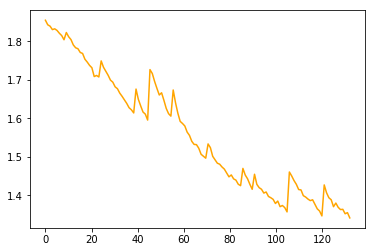
\includegraphics[width=0.4\textwidth]{pic/cap.png}
	\caption{График зависимости capacity от номера цикла разряда} 
	\label{fig:1}
\end{figure}
\begin{figure}[h!]
	\center
	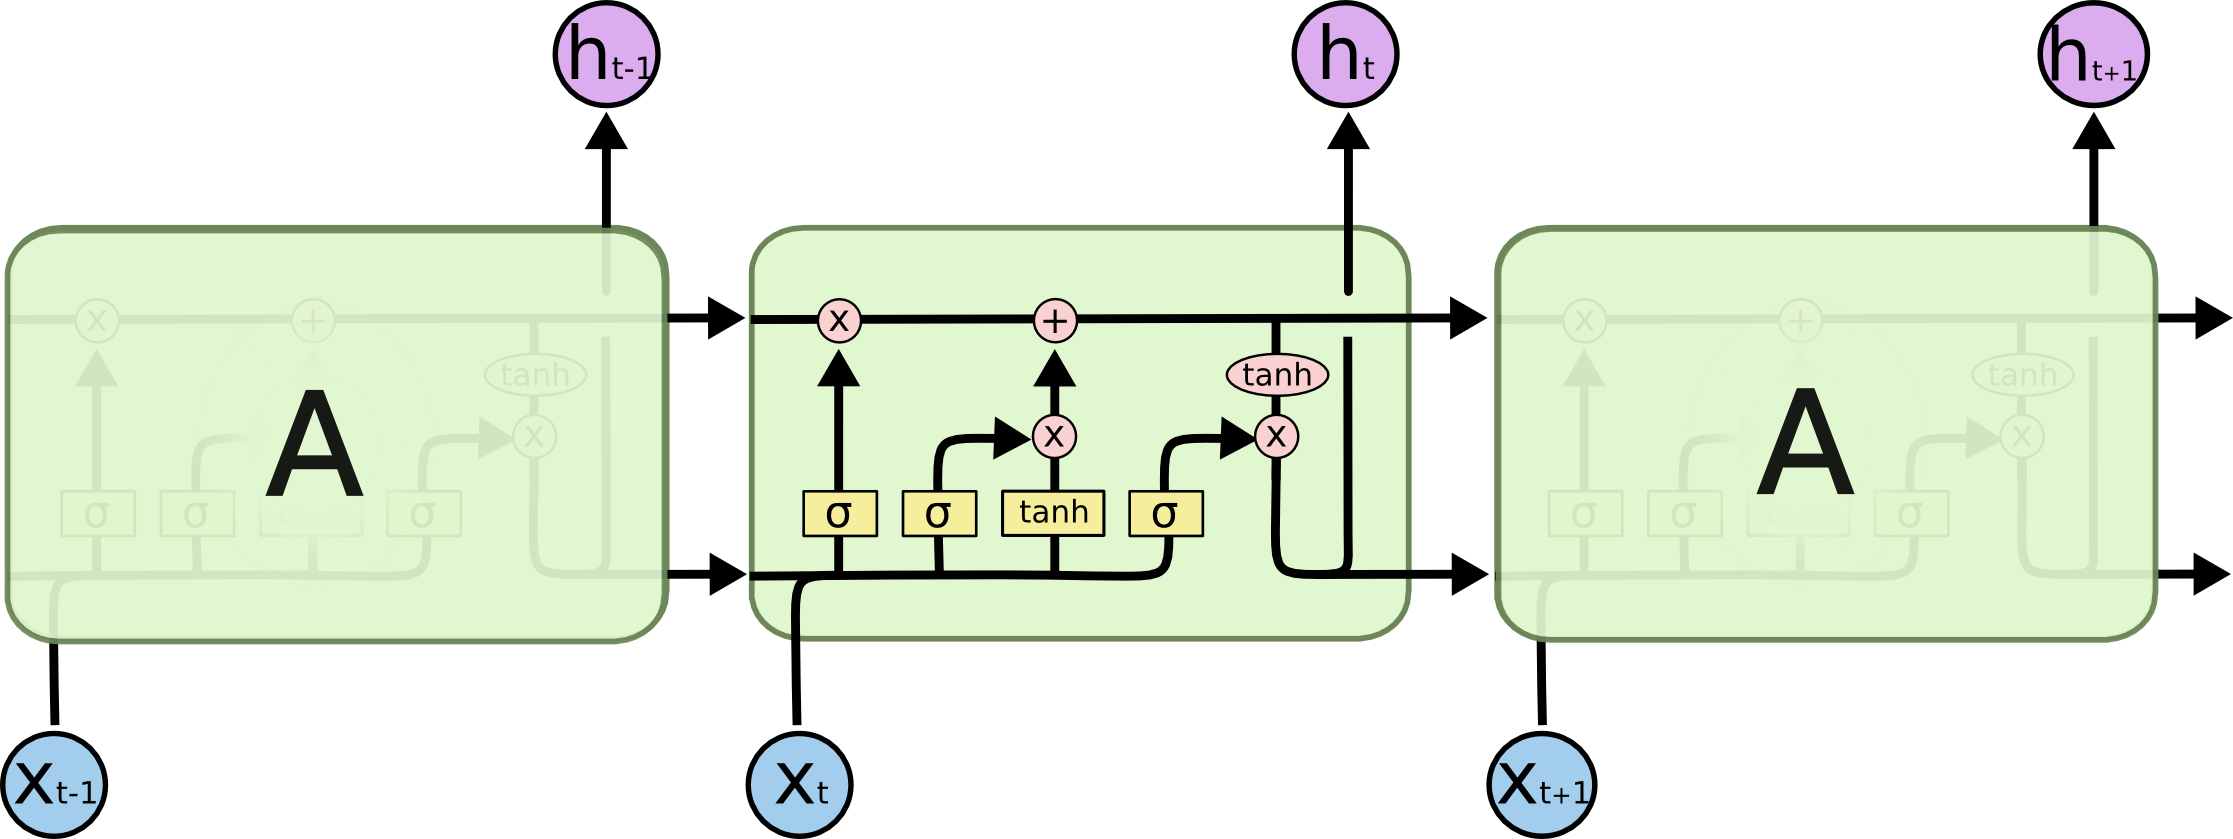
\includegraphics[width=0.7\textwidth]{pic/LSTM3-chain.png}
	\caption{Принцип LSTM рекуррентной нейронной сети} 
	\label{fig:2}
\end{figure}
\newpage
\subsection{Реализация метода}
Программа написана на языке $Python 2$, и в ней использовались библиотеки $keras$, $numpy$, $matplotlib$, $pandas$, $sklearn$ и $scipy$. \\\\
Чуть подробнее об использовании каждой из библиотек:
\begin{itemize}
	\item[$Keras$] Библиотека глубинного обучения с достаточным количеством метрик, оптимизаторов и функций потерь, которая может применяться на основе $Theano$ или $TensorFlow$. Было решено использовать backend $Theano$, чтобы попробовать распараллелить на CUDA, но, к сожалению, имеющаяся видеокарта NVidia GeForce 610M оказалась слишком старой и значительного прироста это не дало, только ускорение в 1.5---2 раза;
	\item[$NumPy$] Библиотека, из которой были использованы numpy-массивы для ускорения работы и упрощения реализации программы;
	\item[$Matplotlib$] Библиотека для построения графиков;
	\item[$Pandas$] Была использована для загрузки .csv датасетов;
	\item[$Sklearn$] Еще одна библиотека, используемая для машинного обучения. Для качества измерения использовались различные метрики из нее;
	\item[$SciPy$] Была нужна для загрузки изначального .mat набора данных.
\end{itemize}
Процесс реализации состоял из следующих этапов:
\begin{enumerate}
	\item Загрузка набора данных: \\
	При помощи метода loadmat из scipy.io был загружен изначальный набор данных циклов батарей. Структура была неудобна для дальнейшего использования, а именно, имела вид: 
	\begin{python}
dataset[fileName][0, 0][0][0][i][3][0][0][k][0][j]
	\end{python}
	где $i$ --- номер цикла, $k$ --- номер вектора в цикле, $j$ --- номер параметра в векторе.
	\item Выбор тренировочного и тестового датасетов:
	 \\ Так как батареи $6$ и $18$ разряжались до одинакового напряжения (2.5 В), было решено выбрать батарею $6$ в качестве тренировочного датасета, а $18$ в качестве тестового датасета.
	\begin{itemize}
		\item Создание тренировочного и тестового датасетов объектов: \\ 
		Поскольку один цикл разряда представлял собой матрицу $Nx6$, где $N$ был от $180$ до $371$, было решено брать 10 равнораспределенных векторов при помощи: \begin{python}
np.linspace(0, numbOfVect-1, 10, dtype=int)
		\end{python} и объединять их в один для каждого цикла. 
		В итоге получилось два набора данных: x\_train ($168x60$) и x\_test ($132x60$);
		\item Создание тренировочного и тестового датасетов целевой переменной: \\ 
		В каждом цикле разряда также содержалось одно значение емкости батареи (capacity). Целью построенной рекуррентной нейронной сети являлось предсказание данного значения по входному вектору состояния цикла разряда батареи. \\
		 Были также созданы 2 набора данных целевой переменной: y\_train ($168x1$) и y\_test ($132x1$);.
	\end{itemize}
	\item Построение модели:\\
	В ходе построения LSTM рекуррентной нейросети были использованы слои: 
	\begin{itemize}
	    \item[] keras.layers.Dense(60, input\_shape=(60,))
	    \item[] keras.layers.Reshape((60,1)))
	    \item[] keras.layers.LSTM(60, return\_sequences=True)
	    \item[] keras.layers.LSTM(60, dropout=0.31, recurrent\_dropout=0.32)
	    \item[] keras.layers.Dense(1)
	\end{itemize}
	В качестве функции потерь (loss) была выбрана среднеквадратическая ошибка, в качестве оптимизатора (optimizer) был выбран  adam, поскольку они оказались наиболее подходящими для решения поставленной задачи.
	\item Выбор оптимальных параметров: \\
	Помимо выбора непосредственно структуры сети, требовалось подобрать оптимальные параметры такие как:
	\begin{itemize} 
		\item Epochs\footnote{Epochs --- количество итераций в процессе обучения. Влияют на степень обученности модели. Большое количество эпох может привести к переобучению на тренировочных данных и, соответственно, плохим результатам на тестовой выборке.}. В качестве оптимального было выбрано значение $21$.
		\item Dropout\footnote{Dropout --- параметр отвечающий за переобучение. Он обнуляет случайную заданную долю признаков и мешает коадаптации весов в слоях.} В качестве оптимального было выбрано значение $0.31$.
		\item В качестве recurrent\_dropout было выбрано $0.32$.
	\end{itemize}
	\item Оценка точности реализованной модели: \\
	После применения реализованной модели к тестовым данным значение функции потерь mean\_square\_error составило $0.000784$.
\end{enumerate}

\newpage

\section{Заключение}
В итоге обученная рекуррентная нейронная сеть предсказала результаты\ref{fig:3} со среднеквадратической ошибкой на тестовых данных, равной $0.000784$
\begin{figure}[h!]
	\center
	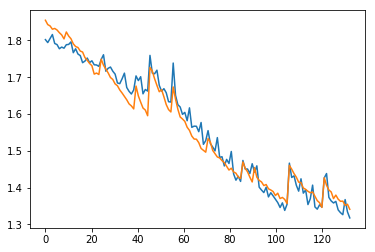
\includegraphics[width=0.5\textwidth]{pic/model.png}
	\caption{Сравнение значений. Желтым --- тестовые данные, синим --- результат предсказания реализованной рекуррентной нейросети} 
	\label{fig:3}
\end{figure}\\
\indentНесмотря на то, что тренировочных данных было мало, обученная реализация модели оказалась способной в достаточной степени предсказывать результат.\\
\indentВ дальнейшем, это исследование может помочь предсказывать оставшееся время жизни батареи по ее состоянию во время цикла разряда.\\\\
Исходный код курсовой работы находится здесь: \href{https://github.com/lysa0/coursework}{https://github.com/lysa0/coursework}

\newpage
\pagestyle{plain}
\section*{Список литературы}
\begin{enumerate}
	\item \href{https://en.wikipedia.org/wiki/Long\_short-term\_memory}{https://en.wikipedia.org/wiki/Long\_short-term\_memory}
	\item \href{http://machinelearningmastery.com/time-series-prediction-lstm-recurrent-neural-networks-python-keras/}{http://machinelearningmastery.com/time-series-prediction-lstm-recurrent-neural-networks-python-keras/}
	\item \href{https://keras.io/metrics/}{https://keras.io/metrics/}
	\item \href{https://keras.io/losses/}{https://keras.io/losses/}
	\item \href{https://keras.io/optimizers/}{https://keras.io/optimizers/}
	\item \href{https://keras.io/models/model/}{https://keras.io/models/model/}
	\item \href{https://ti.arc.nasa.gov/tech/dash/pcoe/prognostic-data-repository/\#battery}{https://ti.arc.nasa.gov/tech/dash/pcoe/prognostic-data-repository/\#battery}
\end{enumerate}
\end{document}
\bye
